\documentclass[compress,red]{beamer}
\mode<presentation>

\usetheme{Montpellier}
% other themes: AnnArbor, Antibes, Bergen, Berkeley, Berlin, Boadilla, boxes, CambridgeUS, Copenhagen, Darmstadt, default, Dresden, Frankfurt, Goettingen,
% Hannover, Ilmenau, JuanLesPins, Luebeck, Madrid, Maloe, Marburg, Montpellier, PaloAlto, Pittsburg, Rochester, Singapore, Szeged, classic

\usecolortheme{beaver}
% color themes: albatross, beaver, beetle, crane, default, dolphin, dove, fly, lily, orchid, rose, seagull, seahorse, sidebartab, structure, whale, wolverine

\usefonttheme{serif}
% font themes: default, professionalfonts, serif, structurebold, structureitalicserif, structuresmallcapsserif

% pdf is displayed in full screen mode automatically
%\hypersetup{pdfpagemode=FullScreen}

\usepackage{subfigure}
\usepackage{multicol}
\usepackage{amsmath}
\usepackage{epsfig}
\usepackage{graphicx}
\usepackage[all,knot]{xy}
\xyoption{arc}
\usepackage{url}
\usepackage{multimedia}
\usepackage{hyperref}
\usepackage{setspace}
\usepackage[retainorgcmds]{IEEEtrantools}
\usepackage{amsfonts, bbm}


\usepackage{etex} % optionally
\usepackage{pgf,tikz}
\usepackage{mathrsfs}
\usepackage{amsfonts, bbm}
\usepackage[]{algorithm2e}
\usetikzlibrary{arrows}

\definecolor{ffxxzr}{rgb}{1.,0.466666666667,0.56862745098}
\definecolor{ffvaxa}{rgb}{1.,0.352941176471,0.478431372549}
\definecolor{ffqqqq}{rgb}{1.,0.,0.}
\definecolor{ffcydc}{rgb}{1.,0.78431372549,0.862745098039}
\definecolor{eqeqeq}{rgb}{0.878431372549,0.878431372549,0.878431372549}
\definecolor{qqqqff}{rgb}{0.,0.,1.}
\definecolor{ttqqqq}{rgb}{0.2,0.,0.}
\definecolor{xdxdff}{rgb}{0.49019607843137253,0.49019607843137253,1.}
\definecolor{qqqqff}{rgb}{0.,0.,1.}
\definecolor{zzttqq}{rgb}{0.6,0.2,0.}
\definecolor{sqsqsq}{rgb}{0.12549019607843137,0.12549019607843137,0.12549019607843137}
\definecolor{darkred}{rgb}{0.8, 0.0, 0.0}
\definecolor{cadmiumgreen}{rgb}{0.0, 0.42, 0.24}
\definecolor{darkspringgreen}{rgb}{0.09, 0.45, 0.27}
\definecolor{green(html/cssgreen)}{rgb}{0.0, 0.5, 0.0}
\definecolor{darkpastelgreen}{rgb}{0.01, 0.75, 0.24}
\definecolor{emerald}{rgb}{0.31, 0.78, 0.47}


\title{Poisson Approximation and the Chen-Stein Method}
\author{Marcin Mider \and Ella Kaye \and Beniamino Hadj-Amar}
\institute{University of Warwick}
\date{November 6th, 2015}

\begin{document}

\frame{
	\titlepage
}

\section{Theory}
\frame{\frametitle{Introduction}

\textcolor{darkred}{Poisson Law of Small Numbers}
\vspace{0.2cm}
		\\Let W $\sim$ Bin($n$, $\lambda/n$), $\quad \lambda > 0$, and let $Z \sim \text{Poi}(\lambda)$.
		
		Then, as $n \rightarrow \infty$:
		
		\begin{center}
			$\mathbb{P}(W = k) \xrightarrow{d} e^{-\lambda}\frac{\lambda^k}{k!} = \mathbb{P}(Z = k),\quad k \in \mathbb{Z}^+$.
		\end{center}
	\vspace{0.5cm}	

	In other words,
	\vspace{0.3cm }
	 
	\centering{$d_{TV}(W, Z)\rightarrow 0, \quad \text{where} \quad d_{TV}(W, Z) =  \sup_{A \subseteq \mathbb{Z}^+}|W(A) - Z(A)|$}
}

\frame{\frametitle{Introduction}
\textcolor{darkred}{Questions}

	\begin{itemize}
		\item Relax assumption of \textit{independence}?
		\item Relax assumption of \textit{identically distributed}?
		
		\item How good is the Poisson approximation?	
	\end{itemize}
	\vspace{0.2cm}
	\textcolor{darkred}{Chen-Stein operator}	
	\begin{equation*}
	A_\lambda g(x) := \lambda g(x + 1) - x g(x),
	\end{equation*}
	\begin{center}
	for every bounded function $g: \mathbb{Z}^+ \rightarrow \mathbb{R}$
	\end{center}
}

\frame{\frametitle{Introduction}
\begin{itemize}
	
	\item<1-> W is distributed as $Z \sim$ Poisson($\lambda$), if and only if
	
	\begin{equation*}
	\mathbb{E}[A_\lambda g(W)] = 0.
	\end{equation*}
	
	\item<2-> We have that 
	\begin{equation*}
	d_{TV}(W, Z) \leq |\mathbb{E}[A_\lambda g(W)]|
	\end{equation*}
	
	\item<3-> To show that W is close to Z, we have to check
	\begin{equation*}
	\mathbb{E}[A_\lambda g(W)] \rightarrow 0.
	\end{equation*}
\end{itemize}

}

\frame{\frametitle{General setting}
Let $X_\alpha,\alpha\in I$, with $I$  a countable index set and:
\begin{equation*}
\mathbbm{P}(X_\alpha=1)=1 - \mathbbm{P}(X_\alpha=0) = p_\alpha.
\end{equation*}
Define $W:=\sum_{\alpha\in I} X_\alpha$, with $\lambda:=\mathbbm{E}[W]$,\\
and a neighbourhood $B_\alpha$
}


\frame{\frametitle{Neighbourhood $B_\alpha$}
\begin{tikzpicture}[line cap=round,line join=round,>=triangle 45,x=1.0cm,y=1.0cm]
\clip(14.3470909091,10.3250909091) rectangle (25.9470909091,18.5069090909);
\begin{scriptsize}
\draw [fill=eqeqeq] (15.26,10.3) circle (3pt);
\draw [fill=eqeqeq] (20.58,12.32) circle (3pt);
\draw [fill=eqeqeq] (24.34,10.74) circle (3pt);
\draw [fill=eqeqeq] (19.,10.) circle (3pt);
\draw [fill=eqeqeq] (16.56,17.22) circle (3pt);
\draw [fill=eqeqeq] (17.3,14.2) circle (3pt);
\draw [fill=eqeqeq] (20.42,14.22) circle (3pt);
\draw [fill=eqeqeq] (24.24,14.4) circle (3pt);
\draw [fill=eqeqeq] (21.0925454545,15.8705454545) circle (3pt);
\draw [fill=eqeqeq] (21.18,16.58) circle (3pt);
\draw [fill=eqeqeq] (21.9,13.46) circle (3pt);
\draw [fill=eqeqeq] (23.2561818182,14.2341818182) circle (3pt);
\draw [fill=eqeqeq] (23.4198181818,12.9614545455) circle (3pt);
\draw [fill=eqeqeq] (22.8925454545,12.4341818182) circle (3pt);
\draw [fill=eqeqeq] (24.5470909091,12.216) circle (3pt);
\draw [fill=eqeqeq] (21.7652727273,11.6887272727) circle (3pt);
\draw [fill=eqeqeq] (22.4016363636,11.1614545455) circle (3pt);
\draw [fill=eqeqeq] (21.9652727273,14.7614545455) circle (3pt);
\draw [fill=eqeqeq] (21.1289090909,15.216) circle (3pt);
\draw [fill=eqeqeq] (20.0925454545,14.7614545455) circle (3pt);
\draw [fill=eqeqeq] (19.6198181818,13.9069090909) circle (3pt);
\draw [fill=eqeqeq] (20.6561818182,13.3614545455) circle (3pt);
\draw [fill=eqeqeq] (22.6016363636,15.8887272727) circle (3pt);
\draw [fill=eqeqeq] (20.3289090909,16.1069090909) circle (3pt);
\end{scriptsize}
\end{tikzpicture}
}

\frame{\frametitle{Neighbourhood $B_\alpha$}
\begin{tikzpicture}[line cap=round,line join=round,>=triangle 45,x=1.0cm,y=1.0cm]
\clip(14.3470909091,10.3250909091) rectangle (25.9470909091,18.5069090909);
\begin{scriptsize}
\draw [fill=eqeqeq] (15.26,10.3) circle (3pt);
\draw [fill=eqeqeq] (20.58,12.32) circle (3pt);
\draw [fill=eqeqeq] (24.34,10.74) circle (3pt);
\draw [fill=eqeqeq] (19.,10.) circle (3pt);
\draw [fill=eqeqeq] (16.56,17.22) circle (3pt);
\draw [fill=eqeqeq] (17.3,14.2) circle (3pt);
\draw [fill=eqeqeq] (20.42,14.22) circle (3pt);
\draw [fill=eqeqeq] (24.24,14.4) circle (3pt);
\draw [fill=darkred] (21.0925454545,15.8705454545) circle (3pt);
\draw[color=darkred] (21.5289090909,16.1796363636) node {$X_\alpha$};
\draw [fill=eqeqeq] (21.18,16.58) circle (3pt);
\draw [fill=eqeqeq] (21.9,13.46) circle (3pt);
\draw [fill=eqeqeq] (23.2561818182,14.2341818182) circle (3pt);
\draw [fill=eqeqeq] (23.4198181818,12.9614545455) circle (3pt);
\draw [fill=eqeqeq] (22.8925454545,12.4341818182) circle (3pt);
\draw [fill=eqeqeq] (24.5470909091,12.216) circle (3pt);
\draw [fill=eqeqeq] (21.7652727273,11.6887272727) circle (3pt);
\draw [fill=eqeqeq] (22.4016363636,11.1614545455) circle (3pt);
\draw [fill=eqeqeq] (21.9652727273,14.7614545455) circle (3pt);
\draw [fill=eqeqeq] (21.1289090909,15.216) circle (3pt);
\draw [fill=eqeqeq] (20.0925454545,14.7614545455) circle (3pt);
\draw [fill=eqeqeq] (19.6198181818,13.9069090909) circle (3pt);
\draw [fill=eqeqeq] (20.6561818182,13.3614545455) circle (3pt);
\draw [fill=eqeqeq] (22.6016363636,15.8887272727) circle (3pt);
\draw [fill=eqeqeq] (20.3289090909,16.1069090909) circle (3pt);
\end{scriptsize}
\end{tikzpicture}
}

\frame{\frametitle{Neighbourhood $B_\alpha$}
\begin{tikzpicture}[line cap=round,line join=round,>=triangle 45,x=1.0cm,y=1.0cm]
\clip(14.3470909091,10.3250909091) rectangle (25.9470909091,18.5069090909);
\begin{scriptsize}
\draw [fill=eqeqeq] (15.26,10.3) circle (3pt);
\draw [fill=ffcydc] (20.58,12.32) circle (3pt);
\draw [fill=eqeqeq] (24.34,10.74) circle (3pt);
\draw [fill=eqeqeq] (19.,10.) circle (3pt);
\draw [fill=eqeqeq] (16.56,17.22) circle (3pt);
\draw [fill=eqeqeq] (17.3,14.2) circle (3pt);
\draw [fill=ffcydc] (20.42,14.22) circle (3pt);
\draw [fill=ffcydc] (24.24,14.4) circle (3pt);
\draw [fill=darkred] (21.0925454545,15.8705454545) circle (3pt);
\draw[color=darkred] (21.5289090909,16.1796363636) node {$X_\alpha$};
\draw [fill=ffvaxa] (21.18,16.58) circle (3pt);
\draw [fill=ffcydc] (21.9,13.46) circle (3pt);
\draw [fill=ffcydc] (23.2561818182,14.2341818182) circle (3pt);
\draw [fill=ffcydc] (23.4198181818,12.9614545455) circle (3pt);
\draw [fill=ffcydc] (22.8925454545,12.4341818182) circle (3pt);
\draw [fill=eqeqeq] (24.5470909091,12.216) circle (3pt);
\draw [fill=eqeqeq] (21.7652727273,11.6887272727) circle (3pt);
\draw [fill=eqeqeq] (22.4016363636,11.1614545455) circle (3pt);
\draw [fill=ffxxzr] (21.9652727273,14.7614545455) circle (3pt);
\draw [fill=ffvaxa] (21.1289090909,15.216) circle (3pt);
\draw [fill=ffxxzr] (20.0925454545,14.7614545455) circle (3pt);
\draw [fill=ffcydc] (19.6198181818,13.9069090909) circle (3pt);
\draw [fill=ffcydc] (20.6561818182,13.3614545455) circle (3pt);
\draw [fill=ffxxzr] (22.6016363636,15.8887272727) circle (3pt);
\draw [fill=ffvaxa] (20.3289090909,16.1069090909) circle (3pt);
\end{scriptsize}
\end{tikzpicture}
}

\frame{\frametitle{Neighbourhood $B_\alpha$}
\begin{tikzpicture}[line cap=round,line join=round,>=triangle 45,x=1.0cm,y=1.0cm]
\clip(14.3470909091,10.3250909091) rectangle (25.9470909091,18.5069090909);
\draw(21.0925454545,15.8705454545) circle (1.62185487117cm);
\begin{scriptsize}
\draw [fill=eqeqeq] (15.26,10.3) circle (3pt);
\draw [fill=ffcydc] (20.58,12.32) circle (3pt);
\draw [fill=eqeqeq] (24.34,10.74) circle (3pt);
\draw [fill=eqeqeq] (19.,10.) circle (3pt);
\draw [fill=eqeqeq] (16.56,17.22) circle (3pt);
\draw [fill=eqeqeq] (17.3,14.2) circle (3pt);
\draw [fill=ffcydc] (20.42,14.22) circle (3pt);
\draw [fill=ffcydc] (24.24,14.4) circle (3pt);
\draw [fill=darkred] (21.0925454545,15.8705454545) circle (3pt);
\draw[color=darkred] (21.5289090909,16.1796363636) node {$X_\alpha$};
\draw [fill=ffvaxa] (21.18,16.58) circle (3pt);
\draw [fill=ffcydc] (21.9,13.46) circle (3pt);
\draw [fill=ffcydc] (23.2561818182,14.2341818182) circle (3pt);
\draw [fill=ffcydc] (23.4198181818,12.9614545455) circle (3pt);
\draw [fill=ffcydc] (22.8925454545,12.4341818182) circle (3pt);
\draw [fill=eqeqeq] (24.5470909091,12.216) circle (3pt);
\draw [fill=eqeqeq] (21.7652727273,11.6887272727) circle (3pt);
\draw [fill=eqeqeq] (22.4016363636,11.1614545455) circle (3pt);
\draw [fill=ffxxzr] (21.9652727273,14.7614545455) circle (3pt);
\draw [fill=ffvaxa] (21.1289090909,15.216) circle (3pt);
\draw [fill=ffxxzr] (20.0925454545,14.7614545455) circle (3pt);
\draw [fill=ffcydc] (19.6198181818,13.9069090909) circle (3pt);
\draw [fill=ffcydc] (20.6561818182,13.3614545455) circle (3pt);
\draw [fill=ffxxzr] (22.6016363636,15.8887272727) circle (3pt);
\draw [fill=ffvaxa] (20.3289090909,16.1069090909) circle (3pt);
\draw[color=black] (20.638,17.0887272727) node {$B_\alpha$};
\end{scriptsize}
\end{tikzpicture}
}

\frame{\frametitle{General setting}
\begin{equation}\label{b_1}
b_1 = \sum_{\alpha\in I}\sum_{\beta\in B_\alpha}p_\alpha p_\beta,
\end{equation}
\begin{equation}\label{b_2}
b_2 = \sum_{\alpha\in I}\sum_{\beta\in B_\alpha \setminus \{\alpha\}}\mathbbm{E}[X_\alpha X_\beta],
\end{equation}
\begin{equation}\label{b_3}
b_3 = \sum_{\alpha\in I}\mathbbm{E}\bigg[\mathbbm{E}[X_\alpha-p_\alpha|\sigma(X_\beta:\beta\notin B_\alpha)]\bigg].
\end{equation}
}


\frame{\frametitle{Chen-Stein bound}
\begin{theorem}
Let $W = \sum_\alpha X_\alpha$, with $\lambda=\mathbbm{E}[W]<\infty$ and let $Z\sim Pois(\lambda)$. Then:
\begin{equation*}
||\mathcal{L}(W)-\mathcal{L}(Z)||_{TV}\leq 2\bigg [ (b_1+b_2)\frac{1-e^{-\lambda}}{\lambda} + b_3 \big(1\wedge \frac{1.4}{\sqrt{\lambda}}\big) \bigg],
\end{equation*}
and
\begin{equation*}
|\mathbbm{P}(W=0)-e^{-\lambda}|\leq (b_1+b_2+b_3)\frac{1-e^{-\lambda}}{\lambda}.
\end{equation*}
\end{theorem}
}


\section{Applications}
\subsection{The Birthday Problem}


\frame{
\begin{figure}[h] 
\centering

\includegraphics[width=1\textwidth]{birthday_cake.jpg}
\label{fig:cake}
\end{figure}
}

\frame{
\begin{itemize}
\item[]<1-> We have $n$ people in the room and we are looking for a $k$-way coincidence.
\item[]<1-> Assume $d$ days in the year, and a uniform distribution for birthdays throughout the year (i.e.\ the probability of being born on any given day is $\frac{1}{d}$). 
\end{itemize}
}

\frame{
\begin{itemize}
\item<1-> Let \{1, \ldots, n\} denote the group of individuals.
\item<1-> Let the index set $I \equiv \{ \alpha \subset  \{1, \ldots, n \} : |\alpha| = k \}$.
\item<2-> Let $X_\alpha$ be a Bernoulli random variable, which takes the value 1 when all the $k$ people indexed by $\alpha$ share a birthday. 
\item<2-> This happens with probability $p_\alpha = (\frac{1}{d})^{k-1} = d^{1-k},\ \forall \alpha $. 
\item<3-> Then $W$, the total number of coincidences, is given by $W = \sum_{\alpha \in I} X_\alpha$,
\item<3-> And $\lambda = \mathbb{E}[W] = \sum_{\alpha \in I} d^{1-k} = {n \choose k} d^{1-k}$.
\item<4-> Approximate $W$ with a Poisson random variable, $Z$, with mean $\lambda$.
\end{itemize}
}

\frame{
\begin{itemize}
\item[]<1-> 
Classic case: $n=23, k=2, d=365$
\item[]<2-> 
\[
\mathbb{P}(W = 0) = \prod_{i=1}^{n-1}\left(1 - \frac{i}{d}\right) = 0.4927
\]
\item[]<3->
\[
\mathbb{P}(Z = 0) = e^{-\lambda} = \exp\left\{- {n \choose k} d^{1-k}\right\} = 0.4999982 
\]
\vspace{0.25cm}
\item[]<4-> The approximation is always conservative when birthdays are uniform.
\end{itemize}
}

\frame{
\begin{itemize}
\item<1-> If $\alpha \cap \beta = \emptyset$, then $X_\alpha$ and $X_\beta$ are independent.
\item<2-> Therefore, take the neighbourhood of dependence to be
\[
B_\alpha = \{\beta \in I : \alpha \cap \beta \neq \emptyset \}.
\]
\item<3-> With this choice,
\[
b_3 = \sum_{\alpha \in I} \mathbb{E}[|\mathbb{E}[X_\alpha - p_\alpha] | \sigma(X_\beta : \beta \notin B_{\alpha}) |]
 = 0.
\]
\end{itemize}
}

\frame{
\begin{IEEEeqnarray*}{rCl}
b_1 & = & \sum_{\alpha \in I} \sum_{\beta \in B_\alpha} p_\alpha p_\beta \\ \\
%& = & | I | | B_\alpha |\ p^2_\alpha \\ \\
& = & {n \choose k} \left\{  {n \choose k} -  {n - k \choose k}      \right\} d^{2-2k} \\ \\ \\
\end{IEEEeqnarray*}
}

\frame{
\begin{itemize}
\item[]<1-> 
\begin{IEEEeqnarray*}{rCl}
%%b_1 & = & \sum_{\alpha \in I} \sum_{\beta \in B_\alpha} p_\alpha p_\beta \\ \\
%%& = & | I | | B_\alpha |\ p^2_\alpha \\ \\
%%& = & {n \choose k} \left\{  {n \choose k} -  {n - k \choose k}      \right\} d^{2-2k} \\ \\ \\
b_2 & = & \sum_{\alpha \in I} \sum_{\beta \in B_\alpha \backslash \{\alpha\}} \mathbbm{E}[X_\alpha X_\beta] \\ \\
%%& = & | I |\sum_{\beta \in B_\alpha \backslash \{\alpha\}} \mathbb{E}[X_\alpha X_\beta] \\
& = & \sum_{j=1}^{k-1} {n \choose k} {k \choose j} {n-k \choose k-j} d^ {\ 1+j-2k}
\end{IEEEeqnarray*}

\item[]<2->
\begin{IEEEeqnarray*}{rCl}
\mathbbm{E}[X_\alpha X_\beta] & = & \mathbbm{P}[X_\alpha = 1,X_\beta = 1] \\
& = &\mathbbm{P}[\text{all people indexed by } \alpha\cup\beta \text{ share same bday}]
\end{IEEEeqnarray*}



\item[]<2-> 
%
%%\begin{columns}
%%\begin{column}{0.5\textwidth}
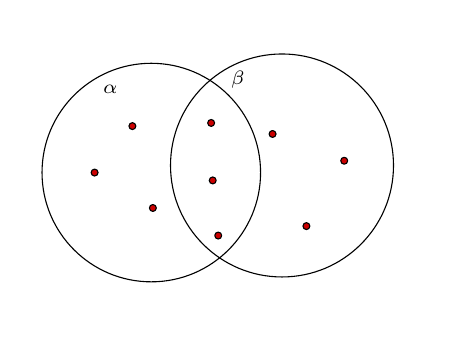
\begin{tikzpicture}[scale = 0.5, line cap=round,line join=round,>=triangle 45,x=1.0cm,y=1.0cm]
\clip(0.96,2.08) rectangle (11.3,9.38);
\draw(4.1,5.7) circle (2.775463925184401cm);
\draw(7.42,5.88) circle (2.831960451701259cm);
\begin{scriptsize}
\draw [fill=darkred] (5.62,6.96) circle (2.5pt);
\draw [fill=darkred] (5.66,5.5) circle (2.5pt);
\draw [fill=darkred] (5.8,4.1) circle (2.5pt);
\draw [fill=darkred] (7.18,6.68) circle (2.5pt);
\draw [fill=darkred] (8.04,4.34) circle (2.5pt);
\draw [fill=darkred] (9.,6.) circle (2.5pt);
\draw [fill=darkred] (3.62,6.88) circle (2.5pt);
\draw [fill=darkred] (4.14,4.8) circle (2.5pt);
\draw [fill=darkred] (2.66,5.7) circle (2.5pt);
\draw[color=black] (3.06,7.82) node {$\alpha$};
\draw[color=black] (6.3,8.06) node {$\beta$};
\end{scriptsize}
\end{tikzpicture}
%%\end{column}
%%
%%\begin{column}{0.5\textwidth}
%%point $\longleftrightarrow$ birthday of particular person
%%\begin{equation*}
%%%\begin{split}
%%%\end{split}
%%\end{equation*}
%%\end{column}
%%\end{columns}
%%
%%
%%
\end{itemize}
%
}

\frame{\frametitle{Bounds as $n$ increases, for fixed $d$}
\begin{figure}[h] 
\centering
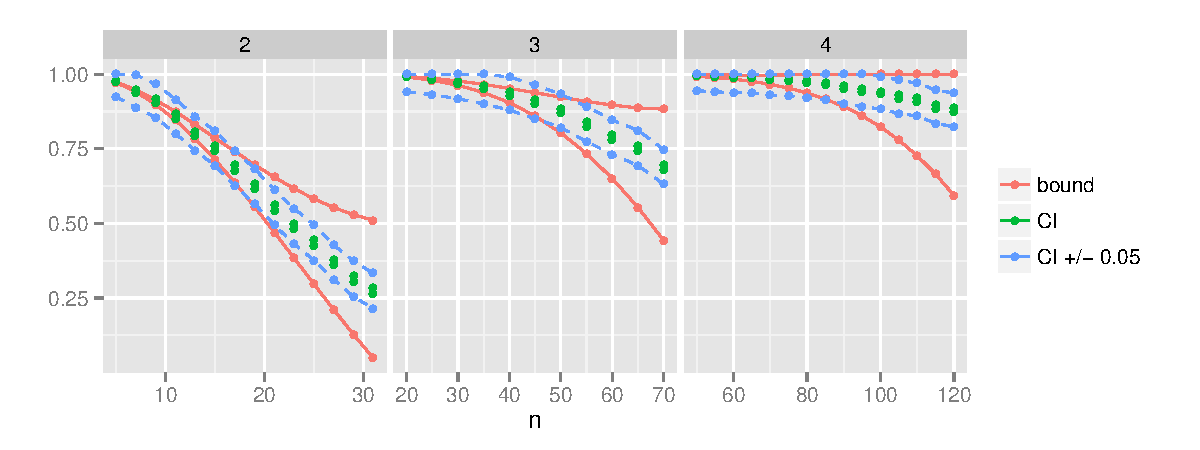
\includegraphics[width=1\textwidth]{graph_n.pdf}
\caption{Simulations for $\mathbb{P}(W=0)$, compared to the bounds given by the Chen-Stein method. The bounds are good when they (the red lines) are inside the blue lines, i.e.\ no more that 0.05 away from the simulated values. The bounds widen as $n$ increases, for fixed $d=365$, for each of $k=2,3,4$.}
\label{fig:graph_n}
\end{figure}
}

\frame{\frametitle{Bounds as $d$ increases, for fixed $n$}
\begin{figure}[h] 
\centering
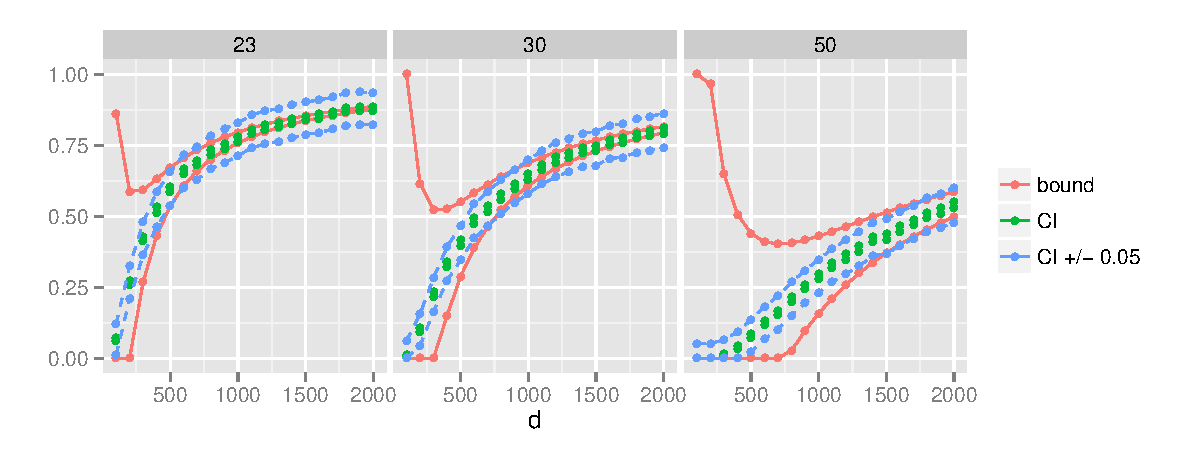
\includegraphics[width=1\textwidth]{graph_d.pdf}
\caption{Simulations for $\mathbb{P}(W=0)$, compared to the bounds given by the Chen-Stein method. The bounds are good when they (the red lines) are inside the blue lines, i.e.\ no more that 0.05 away from the simulated values. The bounds widen as $d$ increases, for fixed $k=2$, for each of $n=23, 30, 50$.}
\label{fig:graph_d}
\end{figure}
}


\frame{
\begin{itemize}
\item<1-> Take both $n, d \to \infty$. We do this in such a way that $\lambda/1$ stays bounded away from zero and $\infty$, denoted $\lambda \asymp 1$.
\item<2-> This implies that $n^k \asymp d^{k-1}$ (since $\lambda = {n \choose k} d^{1-k}$).
\item <3-> We fixed the ratio $\frac{n^k}{d^{1-k}}$ at 1.45 (the value it takes in the classic case).
\item<4-> The order of the Chen-Stein bound here is the same as the order of $b_2$, which is
\[
n^{k+1}d^{-k} \asymp n^{-1/(k-1)}.
\]
Thus the Chen-Stein method yields that the total variation distance decays at a rate no slower than $O(n^{-1/(k-1)})$
\end{itemize}
}

\frame{\frametitle{Bounds as $n, d \to \infty$}
\begin{figure}[h] 
\centering
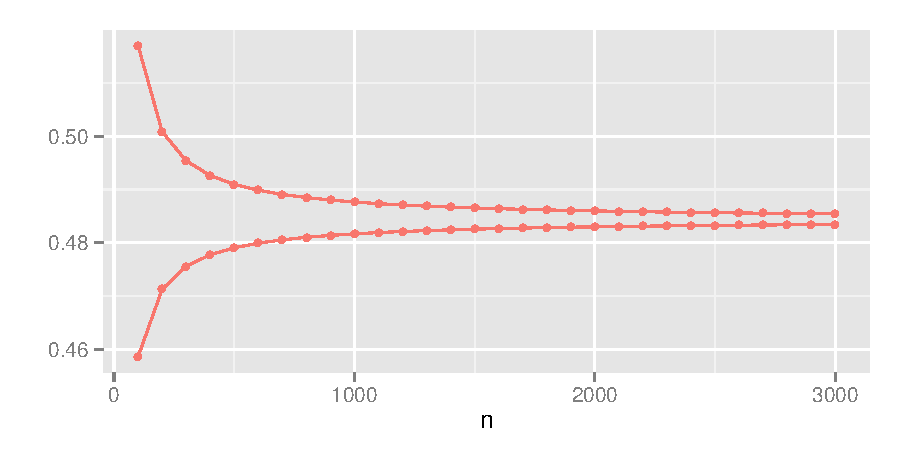
\includegraphics[width=1\textwidth]{graph_nd.pdf}
\caption{The Chen-Stein bounds on the distance between $\mathbb{P}(W=0)$ and $\mathbb{P}(Z=0)$ as $n$ increases, keeping the ratio $\frac{n^k}{d^{1-k}}$ constant at 1.45}
\label{fig:graph_nd}
\end{figure}
}


\subsection{Longest Head Run} \label{sec:LHR}
\frame{\frametitle{The Length of the Longest Head Run}
	Consider
	\begin{itemize}
		\item $n$ independent coin tosses $C_i \sim$ Ber($p$)
		\item test length $t$
	\end{itemize}
	\vspace{0.2cm}
	\textcolor{darkred}{Goal}:
	What's the probability of  having a run of \textit{at least} $t$ heads in the sequence of tosses?
	
	\vspace{0.2cm} 
	Runs could occur in \textbf{clumps}:
	\vspace{0.2cm}
	\begin{itemize}
		
		
		
		\item[-] [0, 1, 0, \textcolor{darkred}{1}, \textcolor{darkred}{1},
		\textcolor{darkred}{1},
		\textcolor{black}{1}, 0, 1]
		
		\vspace{0.2cm}
		\item[-] [0, 1, 0, \textcolor{black}{1}, \textcolor{darkred}{1},
		\textcolor{darkred}{1},
		\textcolor{darkred}{1}, 0, 1]
	\end{itemize}
	\vspace{0.2cm}
	We count only the first sequence of $t$ heads.
}


\frame{\frametitle{The Length of the Longest Head Run}
	
	
	
	\begin{itemize}
		\item[]<1-> Let's define
		\begin{equation*}
		Y_\alpha = \prod_{i = \alpha}^{\alpha + t -1} C_i.
		\end{equation*}
		\item[]<2-> and de-clump
		\begin{equation*}
		X_\alpha = (1 - C_{\alpha - 1})Y_\alpha, \qquad \text{where } X_1 = Y_1.
		\end{equation*}
		\item[]<3-> Therefore
		\begin{equation*}
		W = \sum_{\alpha \in I}^{}X_\alpha \approx \text{Poi}(\lambda) \quad \text{where } \lambda = \mathbb{E}(W).
		\end{equation*}
		
		\begin{equation*}
		\lambda = p^t[(1-p)(n-1) + 1)].
		\end{equation*}
		
	\end{itemize}
	
}


\frame{\frametitle{The Length of the Longest Head Run}
	
	\begin{itemize}
		\item<1-> Neighbourhood of dependence
		\begin{equation*}
		B_\alpha = \{\beta \in I: |\alpha - \beta | \leq t\}
		\end{equation*}
		\item<2-> $b_3 = 0$
		\begin{equation*}
		\mathbb{E}[X_\alpha - p_\alpha \, | \, \sigma(X_\beta : \beta \notin B_\alpha)] = \mathbb{E}(X_\alpha - p) = 0
		\end{equation*}
		\item<3-> $b_2 = 0$
		\begin{equation*}
		X_\alpha = 1 \iff X_\beta = 0  \quad \forall \quad \beta \in B_\alpha,\, \beta \neq \alpha
		\end{equation*}
		\begin{equation*}
		\mathbb{E}(X_\alpha X_\beta) = 0.
		\end{equation*}
		\vspace{0.1cm}
		
		\item<4-> $b_1 \, < \, \lambda^2(2t + 1)/n + 2\lambda p^t$
	\end{itemize}
	
}


\frame{\frametitle{The Length of the Longest Head Run}
	\textbf{\textcolor{darkred}{Example:}}
	Consider a sequence $n = 110$ coin tosses, $p$ = 0.5.
	\vspace{0.2cm}
	
	``What's the probability of obtaining a run of at least $t = 8$ heads?''
	
	\begin{figure}[htbp]
		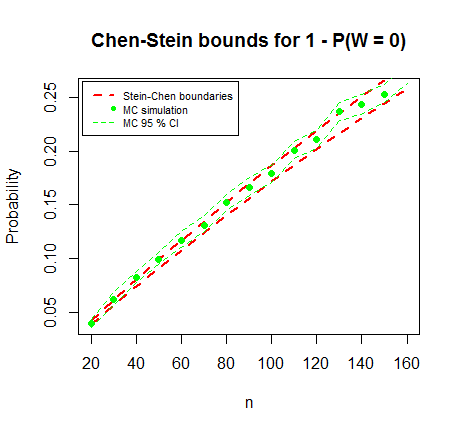
\includegraphics[scale=0.40]{runhead.png}
	\end{figure}
}





\subsection{DNA}
\frame{\frametitle{DNA example}
\begin{tikzpicture}[line cap=round,line join=round,>=triangle 45,x=1.0cm,y=1.0cm]
\clip(4.920405860564847,10.001632527706288) rectangle (14.42949676965571,17.983450709524412);
\draw (5.18,16.86)-- (5.58,16.86);
\draw (5.58,16.86)-- (5.98,16.86);
\draw (5.98,16.86)-- (6.38,16.86);
\draw (6.38,16.86)-- (6.78,16.86);
\draw (6.78,16.86)-- (7.18,16.86);
\draw (7.18,16.86)-- (7.58,16.86);
\draw (7.58,16.86)-- (7.98,16.86);
\draw (7.98,16.86)-- (8.38,16.86);
\draw (8.38,16.86)-- (8.78,16.86);
\draw (8.78,16.86)-- (9.18,16.86);
\draw (9.18,16.86)-- (9.58,16.86);
\draw (9.58,16.86)-- (9.98,16.86);
\draw (9.98,16.86)-- (10.38,16.86);
\draw (10.38,16.86)-- (10.78,16.86);
\draw (10.78,16.86)-- (11.18,16.86);
\draw (11.18,16.86)-- (11.58,16.86);
\draw (11.58,16.86)-- (11.98,16.86);
\draw (13.18,16.86)-- (13.58,16.86);
\draw (13.58,16.86)-- (13.98,16.86);
\begin{scriptsize}
\draw [fill=qqqqff] (5.18,16.86) circle (2.5pt);
\draw[color=qqqqff] (5.302224042383027,17.183450709524415) node {$A$};
\draw [fill=xdxdff] (5.58,16.86) circle (2.5pt);
\draw[color=xdxdff] (5.702224042383024,17.183450709524415) node {$C$};
\draw [fill=xdxdff] (5.98,16.86) circle (2.5pt);
\draw[color=xdxdff] (6.102224042383023,17.183450709524415) node {$T$};
\draw [fill=xdxdff] (6.38,16.86) circle (2.5pt);
\draw[color=xdxdff] (6.502224042383021,17.183450709524415) node {$T$};
\draw [fill=xdxdff] (6.78,16.86) circle (2.5pt);
\draw[color=xdxdff] (6.902224042383018,17.183450709524415) node {$G$};
\draw [fill=xdxdff] (7.18,16.86) circle (2.5pt);
\draw[color=xdxdff] (7.302224042383017,17.183450709524415) node {$G$};
\draw [fill=xdxdff] (7.58,16.86) circle (2.5pt);
\draw[color=xdxdff] (7.702224042383015,17.183450709524415) node {$C$};
\draw [fill=xdxdff] (7.98,16.86) circle (2.5pt);
\draw[color=xdxdff] (8.102224042383012,17.183450709524415) node {$T$};
\draw [fill=xdxdff] (8.38,16.86) circle (2.5pt);
\draw[color=xdxdff] (8.50222404238301,17.183450709524415) node {$A$};
\draw [fill=xdxdff] (8.78,16.86) circle (2.5pt);
\draw[color=xdxdff] (8.90222404238301,17.183450709524415) node {$C$};
\draw [fill=xdxdff] (9.18,16.86) circle (2.5pt);
\draw[color=xdxdff] (9.302224042383006,17.183450709524415) node {$G$};
\draw [fill=xdxdff] (9.58,16.86) circle (2.5pt);
\draw[color=xdxdff] (9.702224042383005,17.183450709524415) node {$A$};
\draw [fill=xdxdff] (9.98,16.86) circle (2.5pt);
\draw[color=xdxdff] (10.102224042383003,17.183450709524415) node {$T$};
\draw [fill=xdxdff] (10.38,16.86) circle (2.5pt);
\draw[color=xdxdff] (10.502224042383002,17.183450709524415) node {$A$};
\draw [fill=xdxdff] (10.78,16.86) circle (2.5pt);
\draw[color=xdxdff] (10.902224042382999,17.183450709524415) node {$C$};
\draw [fill=xdxdff] (11.18,16.86) circle (2.5pt);
\draw[color=xdxdff] (11.302224042382997,17.183450709524415) node {$T$};
\draw [fill=xdxdff] (11.58,16.86) circle (2.5pt);
\draw[color=xdxdff] (11.702224042382996,17.183450709524415) node {$G$};
\draw [fill=xdxdff] (11.98,16.86) circle (2.5pt);
\draw[color=xdxdff] (12.102224042382993,17.183450709524415) node {$G$};
\draw [fill=ttqqqq] (12.38,16.86) circle (1.5pt);
\draw [fill=ttqqqq] (12.78,16.86) circle (1.5pt);
\draw [fill=xdxdff] (13.18,16.86) circle (2.5pt);
\draw[color=xdxdff] (13.302224042382989,17.183450709524415) node {$C$};
\draw [fill=xdxdff] (13.58,16.86) circle (2.5pt);
\draw[color=xdxdff] (13.702224042382985,17.183450709524415) node {$A$};
\draw [fill=xdxdff] (13.98,16.86) circle (2.5pt);
\draw[color=xdxdff] (14.102224042382984,17.183450709524415) node {$T$};
\draw [fill=ttqqqq] (12.582067124052664,16.86) circle (1.5pt);
\end{scriptsize}
\end{tikzpicture}
}

\frame{\frametitle{DNA example}
\begin{tikzpicture}[line cap=round,line join=round,>=triangle 45,x=1.0cm,y=1.0cm]
\clip(4.920405860564846,10.001632527706287) rectangle (14.429496769655712,17.983450709524412);
\draw (5.18,16.86)-- (5.58,16.86);
\draw (5.58,16.86)-- (5.98,16.86);
\draw (5.98,16.86)-- (6.38,16.86);
\draw (6.38,16.86)-- (6.78,16.86);
\draw (6.78,16.86)-- (7.18,16.86);
\draw (7.18,16.86)-- (7.58,16.86);
\draw (7.58,16.86)-- (7.98,16.86);
\draw (7.98,16.86)-- (8.38,16.86);
\draw (8.38,16.86)-- (8.78,16.86);
\draw (8.78,16.86)-- (9.18,16.86);
\draw (9.18,16.86)-- (9.58,16.86);
\draw (9.58,16.86)-- (9.98,16.86);
\draw (9.98,16.86)-- (10.38,16.86);
\draw (10.38,16.86)-- (10.78,16.86);
\draw (10.78,16.86)-- (11.18,16.86);
\draw (11.18,16.86)-- (11.58,16.86);
\draw (11.58,16.86)-- (11.98,16.86);
\draw (13.18,16.86)-- (13.58,16.86);
\draw (13.58,16.86)-- (13.98,16.86);
\draw (7.011314951473927,17.856177982251683)-- (7.011314951473927,15.765268891342608);
\draw (8.9931331332921,17.856177982251687)-- (8.956769496928464,15.67435980043352);
\draw (11.029496769655728,17.874359800433503)-- (11.029496769655728,15.656177982251702);
\draw (13.39313313329208,17.856177982251687)-- (13.411314951473898,15.656177982251702);
\begin{scriptsize}
\draw [fill=qqqqff] (5.18,16.86) circle (2.5pt);
\draw[color=qqqqff] (5.302224042383027,17.18345070952442) node {$A$};
\draw [fill=xdxdff] (5.58,16.86) circle (2.5pt);
\draw[color=xdxdff] (5.702224042383024,17.18345070952442) node {$C$};
\draw [fill=xdxdff] (5.98,16.86) circle (2.5pt);
\draw[color=xdxdff] (6.102224042383023,17.18345070952442) node {$T$};
\draw [fill=xdxdff] (6.38,16.86) circle (2.5pt);
\draw[color=xdxdff] (6.502224042383021,17.18345070952442) node {$T$};
\draw [fill=xdxdff] (6.78,16.86) circle (2.5pt);
\draw[color=xdxdff] (6.902224042383019,17.18345070952442) node {$G$};
\draw [fill=xdxdff] (7.18,16.86) circle (2.5pt);
\draw[color=xdxdff] (7.302224042383017,17.18345070952442) node {$G$};
\draw [fill=xdxdff] (7.58,16.86) circle (2.5pt);
\draw[color=xdxdff] (7.7022240423830155,17.18345070952442) node {$C$};
\draw [fill=xdxdff] (7.98,16.86) circle (2.5pt);
\draw[color=xdxdff] (8.102224042383014,17.18345070952442) node {$T$};
\draw [fill=xdxdff] (8.38,16.86) circle (2.5pt);
\draw[color=xdxdff] (8.50222404238301,17.18345070952442) node {$A$};
\draw [fill=xdxdff] (8.78,16.86) circle (2.5pt);
\draw[color=xdxdff] (8.90222404238301,17.18345070952442) node {$C$};
\draw [fill=xdxdff] (9.18,16.86) circle (2.5pt);
\draw[color=xdxdff] (9.302224042383008,17.18345070952442) node {$G$};
\draw [fill=xdxdff] (9.58,16.86) circle (2.5pt);
\draw[color=xdxdff] (9.702224042383007,17.18345070952442) node {$A$};
\draw [fill=xdxdff] (9.98,16.86) circle (2.5pt);
\draw[color=xdxdff] (10.102224042383005,17.18345070952442) node {$T$};
\draw [fill=xdxdff] (10.38,16.86) circle (2.5pt);
\draw[color=xdxdff] (10.502224042383004,17.18345070952442) node {$A$};
\draw [fill=xdxdff] (10.78,16.86) circle (2.5pt);
\draw[color=xdxdff] (10.902224042383002,17.18345070952442) node {$C$};
\draw [fill=xdxdff] (11.18,16.86) circle (2.5pt);
\draw[color=xdxdff] (11.302224042383,17.18345070952442) node {$T$};
\draw [fill=xdxdff] (11.58,16.86) circle (2.5pt);
\draw[color=xdxdff] (11.702224042382998,17.18345070952442) node {$G$};
\draw [fill=xdxdff] (11.98,16.86) circle (2.5pt);
\draw[color=xdxdff] (12.102224042382996,17.18345070952442) node {$G$};
\draw [fill=ttqqqq] (12.38,16.86) circle (1.5pt);
\draw [fill=ttqqqq] (12.78,16.86) circle (1.5pt);
\draw [fill=xdxdff] (13.18,16.86) circle (2.5pt);
\draw[color=xdxdff] (13.30222404238299,17.18345070952442) node {$C$};
\draw [fill=xdxdff] (13.58,16.86) circle (2.5pt);
\draw[color=xdxdff] (13.702224042382989,17.18345070952442) node {$A$};
\draw [fill=xdxdff] (13.98,16.86) circle (2.5pt);
\draw[color=xdxdff] (14.102224042382987,17.18345070952442) node {$T$};
\draw [fill=ttqqqq] (12.582067124052664,16.86) circle (1.5pt);
\end{scriptsize}
\end{tikzpicture}
}

\frame{\frametitle{DNA example}
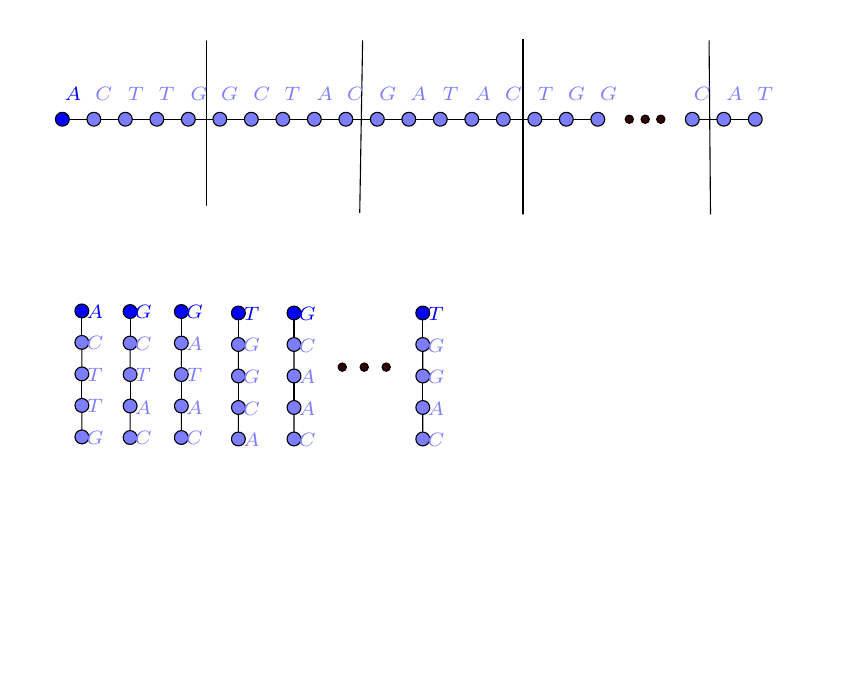
\begin{tikzpicture}[line cap=round,line join=round,>=triangle 45,x=1.0cm,y=1.0cm]
\clip(4.739552456505571,9.865135170235616) rectangle (14.885893919920157,18.023091035508582);
\draw (5.18,16.86)-- (5.58,16.86);
\draw (5.58,16.86)-- (5.98,16.86);
\draw (5.98,16.86)-- (6.38,16.86);
\draw (6.38,16.86)-- (6.78,16.86);
\draw (6.78,16.86)-- (7.18,16.86);
\draw (7.18,16.86)-- (7.58,16.86);
\draw (7.58,16.86)-- (7.98,16.86);
\draw (7.98,16.86)-- (8.38,16.86);
\draw (8.38,16.86)-- (8.78,16.86);
\draw (8.78,16.86)-- (9.18,16.86);
\draw (9.18,16.86)-- (9.58,16.86);
\draw (9.58,16.86)-- (9.98,16.86);
\draw (9.98,16.86)-- (10.38,16.86);
\draw (10.38,16.86)-- (10.78,16.86);
\draw (10.78,16.86)-- (11.18,16.86);
\draw (11.18,16.86)-- (11.58,16.86);
\draw (11.58,16.86)-- (11.98,16.86);
\draw (13.18,16.86)-- (13.58,16.86);
\draw (13.58,16.86)-- (13.98,16.86);
\draw (7.011314951473927,17.856177982251683)-- (7.011314951473927,15.765268891342608);
\draw (8.9931331332921,17.856177982251687)-- (8.956769496928464,15.67435980043352);
\draw (11.029496769655728,17.874359800433503)-- (11.029496769655728,15.656177982251702);
\draw (13.39313313329208,17.856177982251687)-- (13.411314951473898,15.656177982251702);
\draw (5.4276119667519085,14.425725484796256)-- (5.4276119667519085,14.025725484796256);
\draw (5.428160350118287,13.625725860701829)-- (5.4276119667519085,14.025725484796256);
\draw (5.428160350118283,13.225725860701829)-- (5.428160350118287,13.625725860701829);
\draw (5.428160350118283,13.225725860701829)-- (5.427679105125692,12.825726150197863);
\draw (6.040365464635647,14.417980698690917)-- (6.040365464635647,14.017980698690916);
\draw (6.040913848002026,13.61798107459649)-- (6.040365464635647,14.017980698690916);
\draw (6.040913848002021,13.217981074596489)-- (6.040913848002026,13.61798107459649);
\draw (6.040913848002021,13.217981074596489)-- (6.04043260300943,12.817981364092523);
\draw (6.690771968700684,14.417980698690917)-- (6.690771968700684,14.017980698690916);
\draw (6.691320352067063,13.61798107459649)-- (6.690771968700684,14.017980698690916);
\draw (6.691320352067058,13.217981074596489)-- (6.691320352067063,13.61798107459649);
\draw (6.691320352067058,13.217981074596489)-- (6.690839107074467,12.817981364092523);
\draw (7.415510644658869,14.39939765571763)-- (7.415510644658869,13.99939765571763);
\draw (7.416059028025248,13.599398031623203)-- (7.415510644658869,13.99939765571763);
\draw (7.416059028025243,13.199398031623202)-- (7.416059028025248,13.599398031623203);
\draw (7.416059028025243,13.199398031623202)-- (7.415577783032652,12.799398321119236);
\draw (8.121666277643767,14.39939765571763)-- (8.121666277643767,13.99939765571763);
\draw (8.122214661010146,13.599398031623203)-- (8.121666277643767,13.99939765571763);
\draw (8.12221466101014,13.199398031623202)-- (8.122214661010146,13.599398031623203);
\draw (8.12221466101014,13.199398031623202)-- (8.121733416017548,12.799398321119236);
\draw (9.756974059293004,14.39939765571763)-- (9.756974059293004,13.99939765571763);
\draw (9.757522442659383,13.599398031623203)-- (9.756974059293004,13.99939765571763);
\draw (9.757522442659377,13.199398031623202)-- (9.757522442659383,13.599398031623203);
\draw (9.757522442659377,13.199398031623202)-- (9.757041197666785,12.799398321119236);
\begin{scriptsize}
\draw [fill=qqqqff] (5.18,16.86) circle (2.5pt);
\draw[color=qqqqff] (5.315626788677461,17.18685410171067) node {$A$};
\draw [fill=xdxdff] (5.58,16.86) circle (2.5pt);
\draw[color=xdxdff] (5.705870691116484,17.18685410171067) node {$C$};
\draw [fill=xdxdff] (5.98,16.86) circle (2.5pt);
\draw[color=xdxdff] (6.114697636528794,17.18685410171067) node {$T$};
\draw [fill=xdxdff] (6.38,16.86) circle (2.5pt);
\draw[color=xdxdff] (6.504941538967816,17.18685410171067) node {$T$};
\draw [fill=xdxdff] (6.78,16.86) circle (2.5pt);
\draw[color=xdxdff] (6.9137684843801255,17.18685410171067) node {$G$};
\draw [fill=xdxdff] (7.18,16.86) circle (2.5pt);
\draw[color=xdxdff] (7.3040123868191476,17.18685410171067) node {$G$};
\draw [fill=xdxdff] (7.58,16.86) circle (2.5pt);
\draw[color=xdxdff] (7.712839332231457,17.18685410171067) node {$C$};
\draw [fill=xdxdff] (7.98,16.86) circle (2.5pt);
\draw[color=xdxdff] (8.10308323467048,17.18685410171067) node {$T$};
\draw [fill=xdxdff] (8.38,16.86) circle (2.5pt);
\draw[color=xdxdff] (8.51191018008279,17.18685410171067) node {$A$};
\draw [fill=xdxdff] (8.78,16.86) circle (2.5pt);
\draw[color=xdxdff] (8.902154082521811,17.18685410171067) node {$C$};
\draw [fill=xdxdff] (9.18,16.86) circle (2.5pt);
\draw[color=xdxdff] (9.31098102793412,17.18685410171067) node {$G$};
\draw [fill=xdxdff] (9.58,16.86) circle (2.5pt);
\draw[color=xdxdff] (9.701224930373144,17.18685410171067) node {$A$};
\draw [fill=xdxdff] (9.98,16.86) circle (2.5pt);
\draw[color=xdxdff] (10.110051875785453,17.18685410171067) node {$T$};
\draw [fill=xdxdff] (10.38,16.86) circle (2.5pt);
\draw[color=xdxdff] (10.518878821197763,17.18685410171067) node {$A$};
\draw [fill=xdxdff] (10.78,16.86) circle (2.5pt);
\draw[color=xdxdff] (10.909122723636784,17.18685410171067) node {$C$};
\draw [fill=xdxdff] (11.18,16.86) circle (2.5pt);
\draw[color=xdxdff] (11.317949669049094,17.18685410171067) node {$T$};
\draw [fill=xdxdff] (11.58,16.86) circle (2.5pt);
\draw[color=xdxdff] (11.708193571488117,17.18685410171067) node {$G$};
\draw [fill=xdxdff] (11.98,16.86) circle (2.5pt);
\draw[color=xdxdff] (12.117020516900427,17.18685410171067) node {$G$};
\draw [fill=ttqqqq] (12.38,16.86) circle (1.5pt);
\draw [fill=ttqqqq] (12.78,16.86) circle (1.5pt);
\draw [fill=xdxdff] (13.18,16.86) circle (2.5pt);
\draw[color=xdxdff] (13.30633526719078,17.18685410171067) node {$C$};
\draw [fill=xdxdff] (13.58,16.86) circle (2.5pt);
\draw[color=xdxdff] (13.71516221260309,17.18685410171067) node {$A$};
\draw [fill=xdxdff] (13.98,16.86) circle (2.5pt);
\draw[color=xdxdff] (14.105406115042113,17.18685410171067) node {$T$};
\draw [fill=ttqqqq] (12.582067124052664,16.86) circle (1.5pt);
\draw [fill=qqqqff] (5.4276119667519085,14.425725484796256) circle (2.5pt);
\draw[color=qqqqff] (5.594372433276763,14.408224601129941) node {$A$};
\draw [fill=xdxdff] (5.4276119667519085,14.025725484796256) circle (2.5pt);
\draw[color=xdxdff] (5.594372433276763,14.017980698690915) node {$C$};
\draw [fill=xdxdff] (5.428160350118287,13.625725860701829) circle (2.5pt);
\draw[color=xdxdff] (5.594372433276763,13.609153753278603) node {$T$};
\draw [fill=xdxdff] (5.428160350118283,13.225725860701829) circle (2.5pt);
\draw[color=xdxdff] (5.594372433276763,13.218909850839577) node {$T$};
\draw [fill=xdxdff] (5.427679105125692,12.825726150197863) circle (2.5pt);
\draw[color=xdxdff] (5.594372433276763,12.810082905427265) node {$G$};
\draw [fill=qqqqff] (6.040365464635647,14.417980698690917) circle (2.5pt);
\draw[color=qqqqff] (6.207612851395227,14.408224601129941) node {$G$};
\draw [fill=xdxdff] (6.040365464635647,14.017980698690916) circle (2.5pt);
\draw[color=xdxdff] (6.207612851395227,14.009397655717628) node {$C$};
\draw [fill=xdxdff] (6.040913848002026,13.61798107459649) circle (2.5pt);
\draw[color=xdxdff] (6.207612851395227,13.609153753278603) node {$T$};
\draw [fill=xdxdff] (6.040913848002021,13.217981074596489) circle (2.5pt);
\draw[color=xdxdff] (6.207612851395227,13.20032680786629) node {$A$};
\draw [fill=xdxdff] (6.04043260300943,12.817981364092523) circle (2.5pt);
\draw[color=xdxdff] (6.207612851395227,12.810082905427265) node {$C$};
\draw [fill=qqqqff] (6.690771968700684,14.417980698690917) circle (2.5pt);
\draw[color=qqqqff] (6.858019355460264,14.408224601129941) node {$G$};
\draw [fill=xdxdff] (6.690771968700684,14.017980698690916) circle (2.5pt);
\draw[color=xdxdff] (6.858019355460264,14.009397655717628) node {$A$};
\draw [fill=xdxdff] (6.691320352067063,13.61798107459649) circle (2.5pt);
\draw[color=xdxdff] (6.858019355460264,13.609153753278603) node {$T$};
\draw [fill=xdxdff] (6.691320352067058,13.217981074596489) circle (2.5pt);
\draw[color=xdxdff] (6.858019355460264,13.20032680786629) node {$A$};
\draw [fill=xdxdff] (6.690839107074467,12.817981364092523) circle (2.5pt);
\draw[color=xdxdff] (6.858019355460264,12.810082905427265) node {$C$};
\draw [fill=qqqqff] (7.415510644658869,14.39939765571763) circle (2.5pt);
\draw[color=qqqqff] (7.582758031418449,14.389641558156655) node {$T$};
\draw [fill=xdxdff] (7.415510644658869,13.99939765571763) circle (2.5pt);
\draw[color=xdxdff] (7.582758031418449,14.000814612744341) node {$G$};
\draw [fill=xdxdff] (7.416059028025248,13.599398031623203) circle (2.5pt);
\draw[color=xdxdff] (7.582758031418449,13.590570710305317) node {$G$};
\draw [fill=xdxdff] (7.416059028025243,13.199398031623202) circle (2.5pt);
\draw[color=xdxdff] (7.582758031418449,13.181743764893004) node {$C$};
\draw [fill=xdxdff] (7.415577783032652,12.799398321119236) circle (2.5pt);
\draw[color=xdxdff] (7.582758031418449,12.791499862453977) node {$A$};
\draw [fill=qqqqff] (8.121666277643767,14.39939765571763) circle (2.5pt);
\draw[color=qqqqff] (8.288913664403347,14.389641558156655) node {$G$};
\draw [fill=xdxdff] (8.121666277643767,13.99939765571763) circle (2.5pt);
\draw[color=xdxdff] (8.288913664403347,13.980814612744341) node {$C$};
\draw [fill=xdxdff] (8.122214661010146,13.599398031623203) circle (2.5pt);
\draw[color=xdxdff] (8.288913664403347,13.590570710305317) node {$A$};
\draw [fill=xdxdff] (8.12221466101014,13.199398031623202) circle (2.5pt);
\draw[color=xdxdff] (8.288913664403347,13.181743764893004) node {$A$};
\draw [fill=xdxdff] (8.121733416017548,12.799398321119236) circle (2.5pt);
\draw[color=xdxdff] (8.288913664403347,12.791499862453977) node {$C$};
\draw [fill=qqqqff] (9.756974059293004,14.39939765571763) circle (2.5pt);
\draw[color=qqqqff] (9.924221446052584,14.389641558156655) node {$T$};
\draw [fill=xdxdff] (9.756974059293004,13.99939765571763) circle (2.5pt);
\draw[color=xdxdff] (9.924221446052584,13.980814612744341) node {$G$};
\draw [fill=xdxdff] (9.757522442659383,13.599398031623203) circle (2.5pt);
\draw[color=xdxdff] (9.924221446052584,13.590570710305317) node {$G$};
\draw [fill=xdxdff] (9.757522442659377,13.199398031623202) circle (2.5pt);
\draw[color=xdxdff] (9.924221446052584,13.181743764893004) node {$A$};
\draw [fill=xdxdff] (9.757041197666785,12.799398321119236) circle (2.5pt);
\draw[color=xdxdff] (9.924221446052584,12.791499862453977) node {$C$};
\draw [fill=ttqqqq] (8.73490669576223,13.711825065706012) circle (1.5pt);
\draw [fill=ttqqqq] (9.013652340361533,13.711825065706012) circle (1.5pt);
\draw [fill=ttqqqq] (9.292397984960834,13.711825065706012) circle (1.5pt);
\end{scriptsize}
\end{tikzpicture}
}

\frame{\frametitle{DNA example}
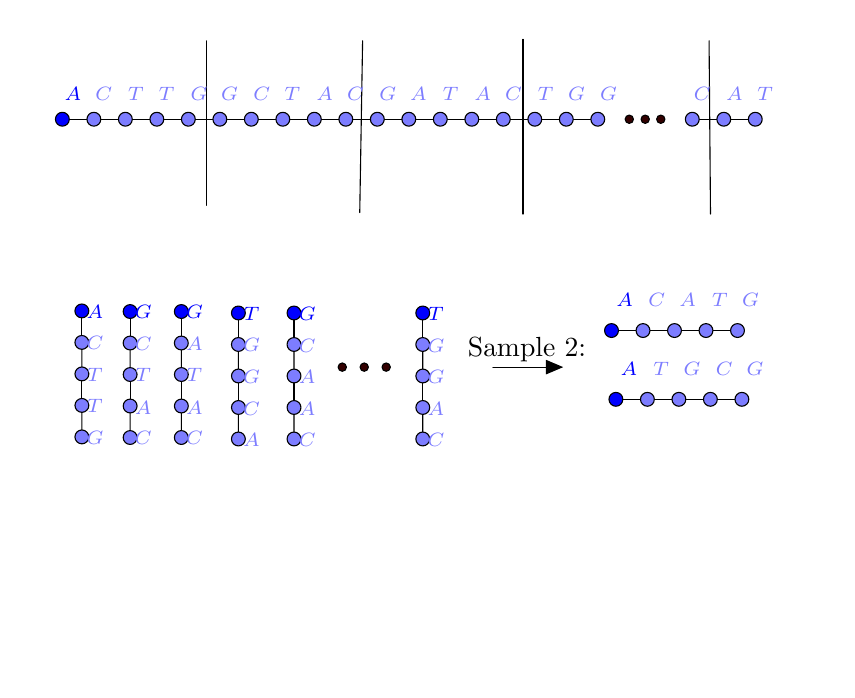
\begin{tikzpicture}[line cap=round,line join=round,>=triangle 45,x=1.0cm,y=1.0cm]
\clip(4.739552456505571,9.865135170235616) rectangle (14.885893919920157,18.023091035508582);
\draw (5.18,16.86)-- (5.58,16.86);
\draw (5.58,16.86)-- (5.98,16.86);
\draw (5.98,16.86)-- (6.38,16.86);
\draw (6.38,16.86)-- (6.78,16.86);
\draw (6.78,16.86)-- (7.18,16.86);
\draw (7.18,16.86)-- (7.58,16.86);
\draw (7.58,16.86)-- (7.98,16.86);
\draw (7.98,16.86)-- (8.38,16.86);
\draw (8.38,16.86)-- (8.78,16.86);
\draw (8.78,16.86)-- (9.18,16.86);
\draw (9.18,16.86)-- (9.58,16.86);
\draw (9.58,16.86)-- (9.98,16.86);
\draw (9.98,16.86)-- (10.38,16.86);
\draw (10.38,16.86)-- (10.78,16.86);
\draw (10.78,16.86)-- (11.18,16.86);
\draw (11.18,16.86)-- (11.58,16.86);
\draw (11.58,16.86)-- (11.98,16.86);
\draw (13.18,16.86)-- (13.58,16.86);
\draw (13.58,16.86)-- (13.98,16.86);
\draw (7.011314951473927,17.856177982251683)-- (7.011314951473927,15.765268891342608);
\draw (8.9931331332921,17.856177982251687)-- (8.956769496928464,15.67435980043352);
\draw (11.029496769655728,17.874359800433503)-- (11.029496769655728,15.656177982251702);
\draw (13.39313313329208,17.856177982251687)-- (13.411314951473898,15.656177982251702);
\draw (5.4276119667519085,14.425725484796256)-- (5.4276119667519085,14.025725484796256);
\draw (5.428160350118287,13.625725860701829)-- (5.4276119667519085,14.025725484796256);
\draw (5.428160350118283,13.225725860701829)-- (5.428160350118287,13.625725860701829);
\draw (5.428160350118283,13.225725860701829)-- (5.427679105125692,12.825726150197863);
\draw (6.040365464635647,14.417980698690917)-- (6.040365464635647,14.017980698690916);
\draw (6.040913848002026,13.61798107459649)-- (6.040365464635647,14.017980698690916);
\draw (6.040913848002021,13.217981074596489)-- (6.040913848002026,13.61798107459649);
\draw (6.040913848002021,13.217981074596489)-- (6.04043260300943,12.817981364092523);
\draw (6.690771968700684,14.417980698690917)-- (6.690771968700684,14.017980698690916);
\draw (6.691320352067063,13.61798107459649)-- (6.690771968700684,14.017980698690916);
\draw (6.691320352067058,13.217981074596489)-- (6.691320352067063,13.61798107459649);
\draw (6.691320352067058,13.217981074596489)-- (6.690839107074467,12.817981364092523);
\draw (7.415510644658869,14.39939765571763)-- (7.415510644658869,13.99939765571763);
\draw (7.416059028025248,13.599398031623203)-- (7.415510644658869,13.99939765571763);
\draw (7.416059028025243,13.199398031623202)-- (7.416059028025248,13.599398031623203);
\draw (7.416059028025243,13.199398031623202)-- (7.415577783032652,12.799398321119236);
\draw (8.121666277643767,14.39939765571763)-- (8.121666277643767,13.99939765571763);
\draw (8.122214661010146,13.599398031623203)-- (8.121666277643767,13.99939765571763);
\draw (8.12221466101014,13.199398031623202)-- (8.122214661010146,13.599398031623203);
\draw (8.12221466101014,13.199398031623202)-- (8.121733416017548,12.799398321119236);
\draw (9.756974059293004,14.39939765571763)-- (9.756974059293004,13.99939765571763);
\draw (9.757522442659383,13.599398031623203)-- (9.756974059293004,13.99939765571763);
\draw (9.757522442659377,13.199398031623202)-- (9.757522442659383,13.599398031623203);
\draw (9.757522442659377,13.199398031623202)-- (9.757041197666785,12.799398321119236);
\draw [->] (10.64896012201077,13.711825065706012) -- (11.540946184728536,13.711825065706012);
\draw (10.20470925093063,14.21356722598476) node[anchor=north west] {Sample 2:};
\draw (12.154186602847,14.176401140038186)-- (12.554186602847,14.176401140038186);
\draw (12.554186602847,14.176401140038186)-- (12.954186602847,14.176401140038186);
\draw (12.954186602847,14.176401140038186)-- (13.354186602847001,14.176401140038186);
\draw (13.354186602847001,14.176401140038186)-- (13.754186602847001,14.176401140038186);
\draw (12.20993573176686,13.302998120293699)-- (12.60993573176686,13.302998120293699);
\draw (12.60993573176686,13.302998120293699)-- (13.009935731766861,13.302998120293699);
\draw (13.009935731766861,13.302998120293699)-- (13.409935731766861,13.302998120293699);
\draw (13.409935731766861,13.302998120293699)-- (13.809935731766862,13.302998120293699);
\begin{scriptsize}
\draw [fill=qqqqff] (5.18,16.86) circle (2.5pt);
\draw[color=qqqqff] (5.315626788677461,17.18685410171067) node {$A$};
\draw [fill=xdxdff] (5.58,16.86) circle (2.5pt);
\draw[color=xdxdff] (5.705870691116484,17.18685410171067) node {$C$};
\draw [fill=xdxdff] (5.98,16.86) circle (2.5pt);
\draw[color=xdxdff] (6.114697636528794,17.18685410171067) node {$T$};
\draw [fill=xdxdff] (6.38,16.86) circle (2.5pt);
\draw[color=xdxdff] (6.504941538967816,17.18685410171067) node {$T$};
\draw [fill=xdxdff] (6.78,16.86) circle (2.5pt);
\draw[color=xdxdff] (6.9137684843801255,17.18685410171067) node {$G$};
\draw [fill=xdxdff] (7.18,16.86) circle (2.5pt);
\draw[color=xdxdff] (7.3040123868191476,17.18685410171067) node {$G$};
\draw [fill=xdxdff] (7.58,16.86) circle (2.5pt);
\draw[color=xdxdff] (7.712839332231457,17.18685410171067) node {$C$};
\draw [fill=xdxdff] (7.98,16.86) circle (2.5pt);
\draw[color=xdxdff] (8.10308323467048,17.18685410171067) node {$T$};
\draw [fill=xdxdff] (8.38,16.86) circle (2.5pt);
\draw[color=xdxdff] (8.51191018008279,17.18685410171067) node {$A$};
\draw [fill=xdxdff] (8.78,16.86) circle (2.5pt);
\draw[color=xdxdff] (8.902154082521811,17.18685410171067) node {$C$};
\draw [fill=xdxdff] (9.18,16.86) circle (2.5pt);
\draw[color=xdxdff] (9.31098102793412,17.18685410171067) node {$G$};
\draw [fill=xdxdff] (9.58,16.86) circle (2.5pt);
\draw[color=xdxdff] (9.701224930373144,17.18685410171067) node {$A$};
\draw [fill=xdxdff] (9.98,16.86) circle (2.5pt);
\draw[color=xdxdff] (10.110051875785453,17.18685410171067) node {$T$};
\draw [fill=xdxdff] (10.38,16.86) circle (2.5pt);
\draw[color=xdxdff] (10.518878821197763,17.18685410171067) node {$A$};
\draw [fill=xdxdff] (10.78,16.86) circle (2.5pt);
\draw[color=xdxdff] (10.909122723636784,17.18685410171067) node {$C$};
\draw [fill=xdxdff] (11.18,16.86) circle (2.5pt);
\draw[color=xdxdff] (11.317949669049094,17.18685410171067) node {$T$};
\draw [fill=xdxdff] (11.58,16.86) circle (2.5pt);
\draw[color=xdxdff] (11.708193571488117,17.18685410171067) node {$G$};
\draw [fill=xdxdff] (11.98,16.86) circle (2.5pt);
\draw[color=xdxdff] (12.117020516900427,17.18685410171067) node {$G$};
\draw [fill=ttqqqq] (12.38,16.86) circle (1.5pt);
\draw [fill=ttqqqq] (12.78,16.86) circle (1.5pt);
\draw [fill=xdxdff] (13.18,16.86) circle (2.5pt);
\draw[color=xdxdff] (13.30633526719078,17.18685410171067) node {$C$};
\draw [fill=xdxdff] (13.58,16.86) circle (2.5pt);
\draw[color=xdxdff] (13.71516221260309,17.18685410171067) node {$A$};
\draw [fill=xdxdff] (13.98,16.86) circle (2.5pt);
\draw[color=xdxdff] (14.105406115042113,17.18685410171067) node {$T$};
\draw [fill=ttqqqq] (12.582067124052664,16.86) circle (1.5pt);
\draw [fill=qqqqff] (5.4276119667519085,14.425725484796256) circle (2.5pt);
\draw[color=qqqqff] (5.594372433276763,14.408224601129941) node {$A$};
\draw [fill=xdxdff] (5.4276119667519085,14.025725484796256) circle (2.5pt);
\draw[color=xdxdff] (5.594372433276763,14.017980698690915) node {$C$};
\draw [fill=xdxdff] (5.428160350118287,13.625725860701829) circle (2.5pt);
\draw[color=xdxdff] (5.594372433276763,13.609153753278603) node {$T$};
\draw [fill=xdxdff] (5.428160350118283,13.225725860701829) circle (2.5pt);
\draw[color=xdxdff] (5.594372433276763,13.218909850839577) node {$T$};
\draw [fill=xdxdff] (5.427679105125692,12.825726150197863) circle (2.5pt);
\draw[color=xdxdff] (5.594372433276763,12.810082905427265) node {$G$};
\draw [fill=qqqqff] (6.040365464635647,14.417980698690917) circle (2.5pt);
\draw[color=qqqqff] (6.207612851395227,14.408224601129941) node {$G$};
\draw [fill=xdxdff] (6.040365464635647,14.017980698690916) circle (2.5pt);
\draw[color=xdxdff] (6.207612851395227,14.009397655717628) node {$C$};
\draw [fill=xdxdff] (6.040913848002026,13.61798107459649) circle (2.5pt);
\draw[color=xdxdff] (6.207612851395227,13.609153753278603) node {$T$};
\draw [fill=xdxdff] (6.040913848002021,13.217981074596489) circle (2.5pt);
\draw[color=xdxdff] (6.207612851395227,13.20032680786629) node {$A$};
\draw [fill=xdxdff] (6.04043260300943,12.817981364092523) circle (2.5pt);
\draw[color=xdxdff] (6.207612851395227,12.810082905427265) node {$C$};
\draw [fill=qqqqff] (6.690771968700684,14.417980698690917) circle (2.5pt);
\draw[color=qqqqff] (6.858019355460264,14.408224601129941) node {$G$};
\draw [fill=xdxdff] (6.690771968700684,14.017980698690916) circle (2.5pt);
\draw[color=xdxdff] (6.858019355460264,14.009397655717628) node {$A$};
\draw [fill=xdxdff] (6.691320352067063,13.61798107459649) circle (2.5pt);
\draw[color=xdxdff] (6.858019355460264,13.609153753278603) node {$T$};
\draw [fill=xdxdff] (6.691320352067058,13.217981074596489) circle (2.5pt);
\draw[color=xdxdff] (6.858019355460264,13.20032680786629) node {$A$};
\draw [fill=xdxdff] (6.690839107074467,12.817981364092523) circle (2.5pt);
\draw[color=xdxdff] (6.858019355460264,12.810082905427265) node {$C$};
\draw [fill=qqqqff] (7.415510644658869,14.39939765571763) circle (2.5pt);
\draw[color=qqqqff] (7.582758031418449,14.389641558156655) node {$T$};
\draw [fill=xdxdff] (7.415510644658869,13.99939765571763) circle (2.5pt);
\draw[color=xdxdff] (7.582758031418449,14.000814612744341) node {$G$};
\draw [fill=xdxdff] (7.416059028025248,13.599398031623203) circle (2.5pt);
\draw[color=xdxdff] (7.582758031418449,13.590570710305317) node {$G$};
\draw [fill=xdxdff] (7.416059028025243,13.199398031623202) circle (2.5pt);
\draw[color=xdxdff] (7.582758031418449,13.181743764893004) node {$C$};
\draw [fill=xdxdff] (7.415577783032652,12.799398321119236) circle (2.5pt);
\draw[color=xdxdff] (7.582758031418449,12.791499862453977) node {$A$};
\draw [fill=qqqqff] (8.121666277643767,14.39939765571763) circle (2.5pt);
\draw[color=qqqqff] (8.288913664403347,14.389641558156655) node {$G$};
\draw [fill=xdxdff] (8.121666277643767,13.99939765571763) circle (2.5pt);
\draw[color=xdxdff] (8.288913664403347,13.980814612744341) node {$C$};
\draw [fill=xdxdff] (8.122214661010146,13.599398031623203) circle (2.5pt);
\draw[color=xdxdff] (8.288913664403347,13.590570710305317) node {$A$};
\draw [fill=xdxdff] (8.12221466101014,13.199398031623202) circle (2.5pt);
\draw[color=xdxdff] (8.288913664403347,13.181743764893004) node {$A$};
\draw [fill=xdxdff] (8.121733416017548,12.799398321119236) circle (2.5pt);
\draw[color=xdxdff] (8.288913664403347,12.791499862453977) node {$C$};
\draw [fill=qqqqff] (9.756974059293004,14.39939765571763) circle (2.5pt);
\draw[color=qqqqff] (9.924221446052584,14.389641558156655) node {$T$};
\draw [fill=xdxdff] (9.756974059293004,13.99939765571763) circle (2.5pt);
\draw[color=xdxdff] (9.924221446052584,13.980814612744341) node {$G$};
\draw [fill=xdxdff] (9.757522442659383,13.599398031623203) circle (2.5pt);
\draw[color=xdxdff] (9.924221446052584,13.590570710305317) node {$G$};
\draw [fill=xdxdff] (9.757522442659377,13.199398031623202) circle (2.5pt);
\draw[color=xdxdff] (9.924221446052584,13.181743764893004) node {$A$};
\draw [fill=xdxdff] (9.757041197666785,12.799398321119236) circle (2.5pt);
\draw[color=xdxdff] (9.924221446052584,12.791499862453977) node {$C$};
\draw [fill=ttqqqq] (8.73490669576223,13.711825065706012) circle (1.5pt);
\draw [fill=ttqqqq] (9.013652340361533,13.711825065706012) circle (1.5pt);
\draw [fill=ttqqqq] (9.292397984960834,13.711825065706012) circle (1.5pt);
\draw [fill=qqqqff] (12.154186602847,14.176401140038186) circle (2.5pt);
\draw[color=qqqqff] (12.32143398960658,14.56664504247721) node {$A$};
\draw [fill=xdxdff] (12.554186602847,14.176401140038186) circle (2.5pt);
\draw[color=xdxdff] (12.73026093501889,14.56664504247721) node {$C$};
\draw [fill=xdxdff] (12.954186602847,14.176401140038186) circle (2.5pt);
\draw[color=xdxdff] (13.120504837457913,14.56664504247721) node {$A$};
\draw [fill=xdxdff] (13.354186602847001,14.176401140038186) circle (2.5pt);
\draw[color=xdxdff] (13.529331782870223,14.56664504247721) node {$T$};
\draw [fill=xdxdff] (13.754186602847001,14.176401140038186) circle (2.5pt);
\draw[color=xdxdff] (13.919575685309244,14.56664504247721) node {$G$};
\draw [fill=qqqqff] (12.20993573176686,13.302998120293699) circle (2.5pt);
\draw[color=qqqqff] (12.37718311852644,13.693242022732726) node {$A$};
\draw [fill=xdxdff] (12.60993573176686,13.302998120293699) circle (2.5pt);
\draw[color=xdxdff] (12.78601006393875,13.693242022732726) node {$T$};
\draw [fill=xdxdff] (13.009935731766861,13.302998120293699) circle (2.5pt);
\draw[color=xdxdff] (13.176253966377773,13.693242022732726) node {$G$};
\draw [fill=xdxdff] (13.409935731766861,13.302998120293699) circle (2.5pt);
\draw[color=xdxdff] (13.585080911790083,13.693242022732726) node {$C$};
\draw [fill=xdxdff] (13.809935731766862,13.302998120293699) circle (2.5pt);
\draw[color=xdxdff] (13.975324814229104,13.693242022732726) node {$G$};
\end{scriptsize}
\end{tikzpicture}
}

\frame{\frametitle{DNA example}
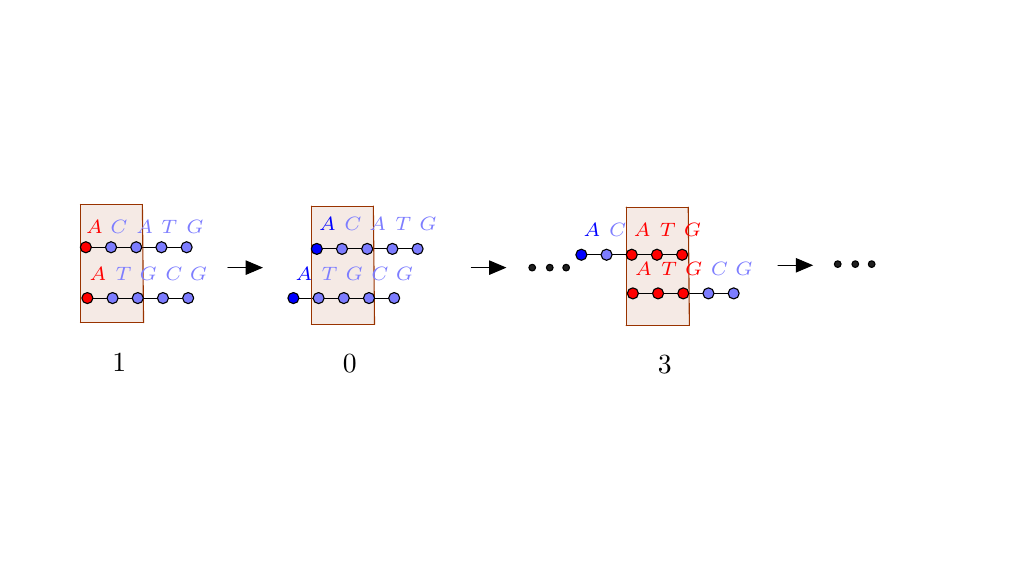
\begin{tikzpicture}[scale = 0.8, line cap=round,line join=round,>=triangle 45,x=1.0cm,y=1.0cm]
\clip(4.25639333920017,12.188015541896485) rectangle (19.68031900702841,20.34597140716945);
\fill[color=zzttqq,fill=zzttqq,fill opacity=0.1] (5.092630272998023,15.663044577901148) -- (6.0961145935555106,15.663044577901148) -- (6.077531550582224,17.53993191820313) -- (5.092630272998023,17.53993191820313) -- cycle;
\fill[color=zzttqq,fill=zzttqq,fill opacity=0.1] (8.759035226599982,15.636820863119372) -- (9.762519547157469,15.636820863119372) -- (9.743936504184182,17.513708203421356) -- (8.759035226599982,17.513708203421356) -- cycle;
\fill[color=zzttqq,fill=zzttqq,fill opacity=0.1] (13.757873786414125,15.618237820146085) -- (14.761358106971615,15.618237820146085) -- (14.742775063998325,17.495125160448072) -- (13.757873786414125,17.495125160448072) -- cycle;
\draw (5.18,16.86)-- (5.58,16.86);
\draw (5.58,16.86)-- (5.98,16.86);
\draw (5.98,16.86)-- (6.38,16.86);
\draw (6.38,16.86)-- (6.78,16.86);
\draw (5.204128530837743,16.053288480340168)-- (5.604128530837744,16.053288480340168);
\draw (5.604128530837744,16.053288480340168)-- (6.004128530837744,16.053288480340168);
\draw (6.004128530837744,16.053288480340168)-- (6.4041285308377445,16.053288480340168);
\draw (6.4041285308377445,16.053288480340168)-- (6.804128530837745,16.053288480340168);
\draw [color=zzttqq] (5.092630272998023,15.663044577901148)-- (6.0961145935555106,15.663044577901148);
\draw [color=zzttqq] (6.0961145935555106,15.663044577901148)-- (6.077531550582224,17.53993191820313);
\draw [color=zzttqq] (6.077531550582224,17.53993191820313)-- (5.092630272998023,17.53993191820313);
\draw [color=zzttqq] (5.092630272998023,17.53993191820313)-- (5.092630272998023,15.663044577901148);
\draw (5.44570808949054,15.328549804381979) node[anchor=north west] {1};
\draw [->] (7.434093687632161,16.536447597645637) -- (7.991584976830764,16.536447597645637);
\draw (8.846404953601958,16.833776285218224)-- (9.246404953601958,16.833776285218224);
\draw (9.246404953601958,16.833776285218224)-- (9.646404953601959,16.833776285218224);
\draw (9.646404953601959,16.833776285218224)-- (10.046404953601959,16.833776285218224);
\draw (10.046404953601959,16.833776285218224)-- (10.44640495360196,16.833776285218224);
\draw (8.474744094136222,16.05328848034017)-- (8.874744094136222,16.05328848034017);
\draw (8.874744094136222,16.05328848034017)-- (9.274744094136222,16.05328848034017);
\draw (9.274744094136222,16.05328848034017)-- (9.674744094136223,16.05328848034017);
\draw (9.674744094136223,16.05328848034017)-- (10.074744094136223,16.05328848034017);
\draw [color=zzttqq] (8.759035226599982,15.636820863119372)-- (9.762519547157469,15.636820863119372);
\draw [color=zzttqq] (9.762519547157469,15.636820863119372)-- (9.743936504184182,17.513708203421356);
\draw [color=zzttqq] (9.743936504184182,17.513708203421356)-- (8.759035226599982,17.513708203421356);
\draw [color=zzttqq] (8.759035226599982,17.513708203421356)-- (8.759035226599982,15.636820863119372);
\draw (9.106567555228086,15.309966761408692) node[anchor=north west] {0};
\draw [->] (11.299366626075814,16.536447597645633) -- (11.856857915274418,16.536447597645633);
\draw (13.046172665564772,16.740861070351787)-- (13.446172665564772,16.740861070351787);
\draw (13.446172665564772,16.740861070351787)-- (13.846172665564772,16.740861070351787);
\draw (13.846172665564772,16.740861070351787)-- (14.246172665564773,16.740861070351787);
\draw (14.246172665564773,16.740861070351787)-- (14.646172665564773,16.740861070351787);
\draw (13.86382655638939,16.12762065223332)-- (14.26382655638939,16.12762065223332);
\draw (14.26382655638939,16.12762065223332)-- (14.66382655638939,16.12762065223332);
\draw (14.66382655638939,16.12762065223332)-- (15.06382655638939,16.12762065223332);
\draw (15.06382655638939,16.12762065223332)-- (15.46382655638939,16.12762065223332);
\draw [color=zzttqq] (13.757873786414125,15.618237820146085)-- (14.761358106971615,15.618237820146085);
\draw [color=zzttqq] (14.761358106971615,15.618237820146085)-- (14.742775063998325,17.495125160448072);
\draw [color=zzttqq] (14.742775063998325,17.495125160448072)-- (13.757873786414125,17.495125160448072);
\draw [color=zzttqq] (13.757873786414125,17.495125160448072)-- (13.757873786414125,15.618237820146085);
\draw (14.105406115042298,15.291383718435405) node[anchor=north west] {3};
\draw [->] (16.16812388507701,16.573613683592217) -- (16.725615174275614,16.573613683592217);
\begin{scriptsize}
\draw [fill=ffqqqq] (5.18,16.86) circle (2.5pt);
\draw[color=ffqqqq] (5.315626788677531,17.186854101710672) node {$A$};
\draw [fill=xdxdff] (5.58,16.86) circle (2.5pt);
\draw[color=xdxdff] (5.705870691116559,17.186854101710672) node {$C$};
\draw [fill=xdxdff] (5.98,16.86) circle (2.5pt);
\draw[color=xdxdff] (6.114697636528874,17.186854101710672) node {$A$};
\draw [fill=xdxdff] (6.38,16.86) circle (2.5pt);
\draw[color=xdxdff] (6.504941538967901,17.186854101710672) node {$T$};
\draw [fill=xdxdff] (6.78,16.86) circle (2.5pt);
\draw[color=xdxdff] (6.913768484380216,17.186854101710672) node {$G$};
\draw [fill=ffqqqq] (5.204128530837743,16.053288480340168) circle (2.5pt);
\draw[color=ffqqqq] (5.371375917597392,16.443532382779196) node {$A$};
\draw [fill=xdxdff] (5.604128530837744,16.053288480340168) circle (2.5pt);
\draw[color=xdxdff] (5.780202863009707,16.443532382779196) node {$T$};
\draw [fill=xdxdff] (6.004128530837744,16.053288480340168) circle (2.5pt);
\draw[color=xdxdff] (6.170446765448735,16.443532382779196) node {$G$};
\draw [fill=xdxdff] (6.4041285308377445,16.053288480340168) circle (2.5pt);
\draw[color=xdxdff] (6.57927371086105,16.443532382779196) node {$C$};
\draw [fill=xdxdff] (6.804128530837745,16.053288480340168) circle (2.5pt);
\draw[color=xdxdff] (6.969517613300077,16.443532382779196) node {$G$};
\draw [fill=qqqqff] (8.846404953601958,16.833776285218224) circle (2.5pt);
\draw[color=qqqqff] (9.013652340361652,17.224020187657246) node {$A$};
\draw [fill=xdxdff] (9.246404953601958,16.833776285218224) circle (2.5pt);
\draw[color=xdxdff] (9.422479285773965,17.224020187657246) node {$C$};
\draw [fill=xdxdff] (9.646404953601959,16.833776285218224) circle (2.5pt);
\draw[color=xdxdff] (9.812723188212992,17.224020187657246) node {$A$};
\draw [fill=xdxdff] (10.046404953601959,16.833776285218224) circle (2.5pt);
\draw[color=xdxdff] (10.221550133625307,17.224020187657246) node {$T$};
\draw [fill=xdxdff] (10.44640495360196,16.833776285218224) circle (2.5pt);
\draw[color=xdxdff] (10.611794036064335,17.224020187657246) node {$G$};
\draw [fill=qqqqff] (8.474744094136222,16.05328848034017) circle (2.5pt);
\draw[color=qqqqff] (8.64199148089591,16.443532382779196) node {$A$};
\draw [fill=xdxdff] (8.874744094136222,16.05328848034017) circle (2.5pt);
\draw[color=xdxdff] (9.050818426308226,16.443532382779196) node {$T$};
\draw [fill=xdxdff] (9.274744094136222,16.05328848034017) circle (2.5pt);
\draw[color=xdxdff] (9.441062328747254,16.443532382779196) node {$G$};
\draw [fill=xdxdff] (9.674744094136223,16.05328848034017) circle (2.5pt);
\draw[color=xdxdff] (9.849889274159567,16.443532382779196) node {$C$};
\draw [fill=xdxdff] (10.074744094136223,16.05328848034017) circle (2.5pt);
\draw[color=xdxdff] (10.240133176598595,16.443532382779196) node {$G$};
\draw [fill=sqsqsq] (12.265684860686726,16.536447597645633) circle (1.5pt);
\draw [fill=sqsqsq] (12.544430505286027,16.536447597645633) circle (1.5pt);
\draw [fill=sqsqsq] (12.804593106912042,16.536447597645633) circle (1.5pt);
\draw [fill=qqqqff] (13.046172665564772,16.740861070351787) circle (2.5pt);
\draw[color=qqqqff] (13.21342005232452,17.131104972790812) node {$A$};
\draw [fill=xdxdff] (13.446172665564772,16.740861070351787) circle (2.5pt);
\draw[color=xdxdff] (13.622246997736836,17.131104972790812) node {$C$};
\draw [fill=ffqqqq] (13.846172665564772,16.740861070351787) circle (2.5pt);
\draw[color=ffqqqq] (14.012490900175862,17.131104972790812) node {$A$};
\draw [fill=ffqqqq] (14.246172665564773,16.740861070351787) circle (2.5pt);
\draw[color=ffqqqq] (14.421317845588177,17.131104972790812) node {$T$};
\draw [fill=ffqqqq] (14.646172665564773,16.740861070351787) circle (2.5pt);
\draw[color=ffqqqq] (14.811561748027206,17.131104972790812) node {$G$};
\draw [fill=ffqqqq] (13.86382655638939,16.12762065223332) circle (2.5pt);
\draw[color=ffqqqq] (14.03107394314915,16.517864554672343) node {$A$};
\draw [fill=ffqqqq] (14.26382655638939,16.12762065223332) circle (2.5pt);
\draw[color=ffqqqq] (14.439900888561464,16.517864554672343) node {$T$};
\draw [fill=ffqqqq] (14.66382655638939,16.12762065223332) circle (2.5pt);
\draw[color=ffqqqq] (14.830144791000492,16.517864554672343) node {$G$};
\draw [fill=xdxdff] (15.06382655638939,16.12762065223332) circle (2.5pt);
\draw[color=xdxdff] (15.238971736412807,16.517864554672343) node {$C$};
\draw [fill=xdxdff] (15.46382655638939,16.12762065223332) circle (2.5pt);
\draw[color=xdxdff] (15.629215638851836,16.517864554672343) node {$G$};
\draw [fill=sqsqsq] (17.11585907671464,16.592196726565504) circle (1.5pt);
\draw [fill=sqsqsq] (17.39460472131394,16.592196726565504) circle (1.5pt);
\draw [fill=sqsqsq] (17.654767322939954,16.592196726565504) circle (1.5pt);
\end{scriptsize}
\end{tikzpicture}
}

\frame{\frametitle{DNA example}
We used a complete chloroplast genome of \emph{Marchantia Polymorpha} (Liverwort), downloaded from GenBank. It consists of one sequence of 121,024 letters.
\begin{figure}
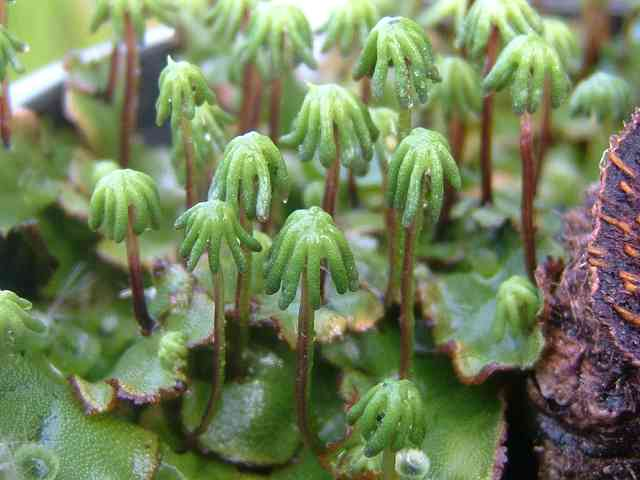
\includegraphics[width=0.5\linewidth]{Liverwort}
\end{figure}
}

\frame{\frametitle{DNA example - algorithm}
\begin{algorithm}[H]
\KwData{Cut the sequence into 236 disjoint \emph{stripes}, each consisting of 512 letters. Discard remaining letters.}
 w.size = 21;  max.matches = vector[200]\;
 \For {$i = 1:200$}{
   draw 2 \emph{stripes} at random, store as str.A and str.B\;
   current.max = 0\;
  \For{each possible placement of window of length w.size on str.A and str.B}{
   current.count = number of matches within window\;
   \If{current.count $>$ current.max}{update current.max\;}
   }
   max.matches[i] = current.max
 }
\end{algorithm}
}

\frame{\frametitle{DNA example}
Suppose that $A_1,A_2,\dots,A_n$ and $B_1,B_2,\dots,B_n$ are two \emph{stripes}, where $A_i,B_i\in\{a,c,t,g\}$, chosen at random according to common distribution $\mu$. Define:
\begin{equation}
M_n(t) = \max_{1\leq i,j\leq n-t+1}\sum_{k=0}^{t-1}\mathbbm{1}_{A_{i+k}=B_{j+k}},
\end{equation}
Then, under some regularity conditions:
\begin{equation}\label{approx_DNA}
\mathbbm{P}[M_n(t)<s]-e^{-n(\frac{s}{t}-p)\mathbbm{P}[Bin(t,p)\geq s]}\rightarrow 0.
\end{equation}
}
\frame{\frametitle{DNA example}
\begin{figure}
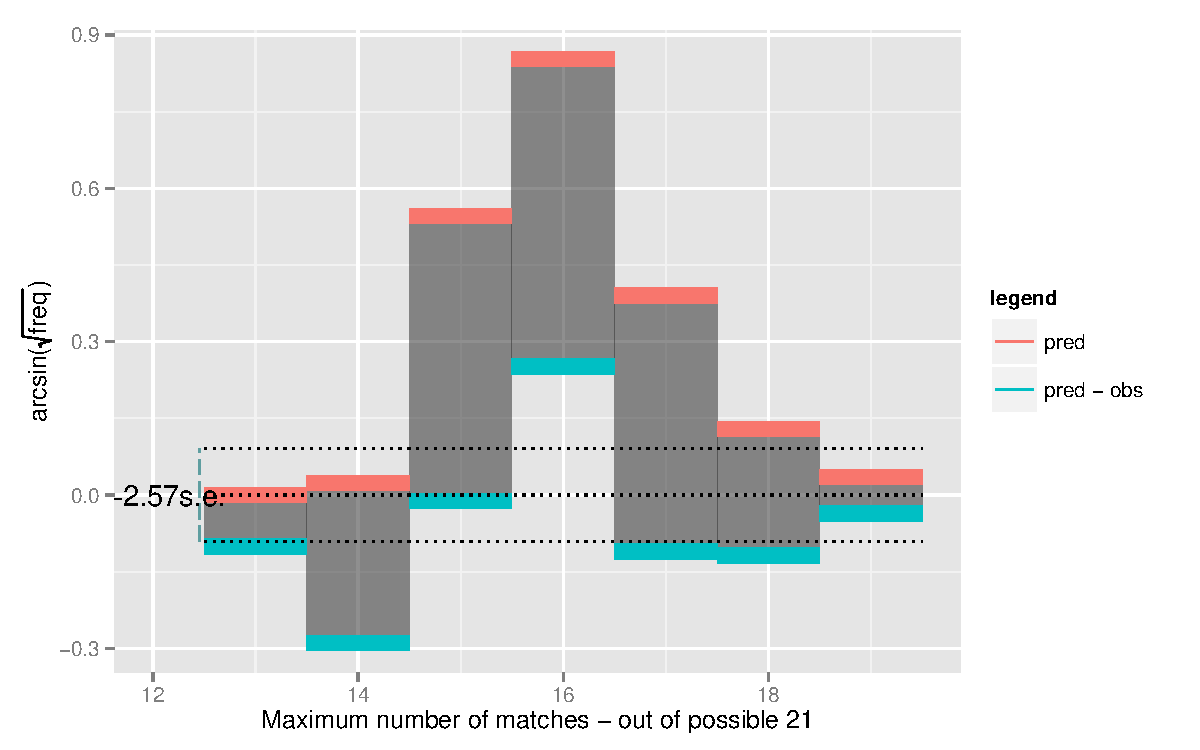
\includegraphics[width=\linewidth]{DNA_prob_liverwort}
\end{figure}
}
\frame{\frametitle{DNA example}
\begin{figure}
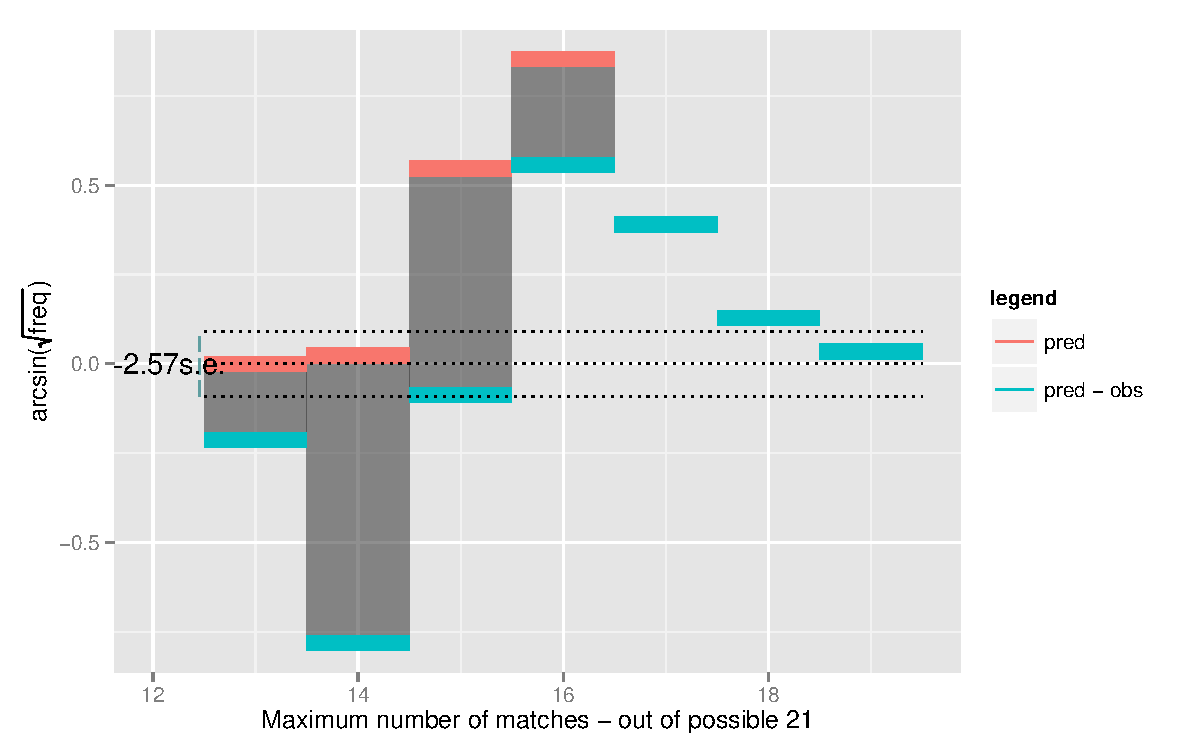
\includegraphics[width=\linewidth]{DNA_prob_sim}
\end{figure}
}





\end{document}